
O circuito característico de um inversor trifásico pode ser ilustrado como na figura \ref{c1it}.

\begin{figure}[h]
\center
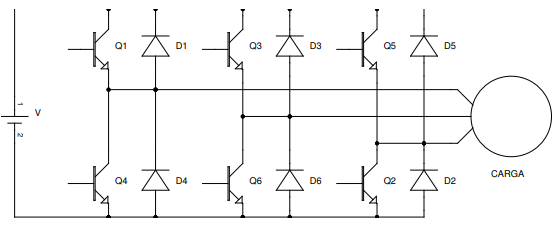
\includegraphics[scale=0.55]{imagens/circuito1_inversor_tri.png}
\caption{Estrutura básica de um inversor trifásico}\label{c1it} 
\caption*{Fonte: Apostila de eletrônica de potência (2015)}
\end{figure}

Serão estudadas duas formas de comutação simples para esse tipo de inversor. A primeira, chamada de comutação seis-pulsos 180º, consiste em acionar cada um dos 6 transistores durante meio ciclo (daí os 180º) igualmente espaçados. O acionamento dos transistores encontra-se ilustrado na figura \ref{g1it}, junto do resultado para a carga em termos de tensão de fase e linha. Veja que a tensão de linha (eficaz) nesse modo de operação é \[
V_R = \sqrt{\frac{2}{3}} V
.\] 

\begin{figure}[h]
\center
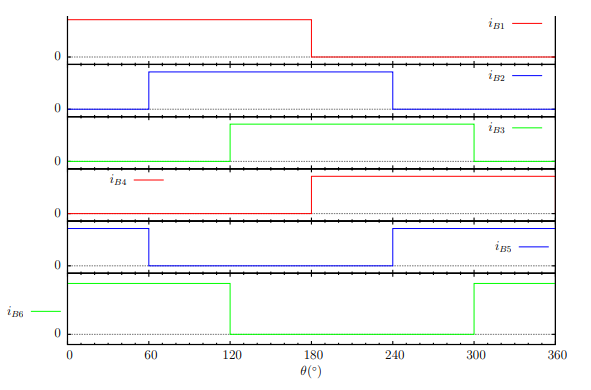
\includegraphics[width=0.32\textwidth]{imagens/grafico1_inversor_tri.png}
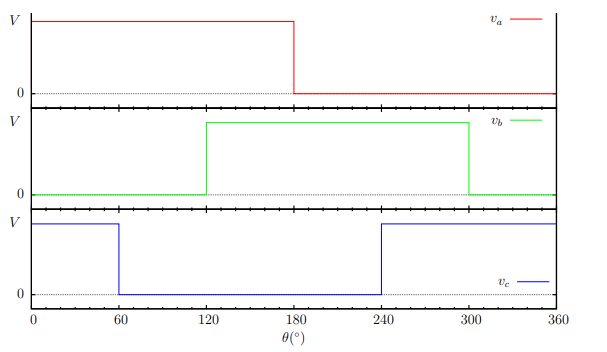
\includegraphics[width=0.32\textwidth]{imagens/grafico2_inversor_tri.png}
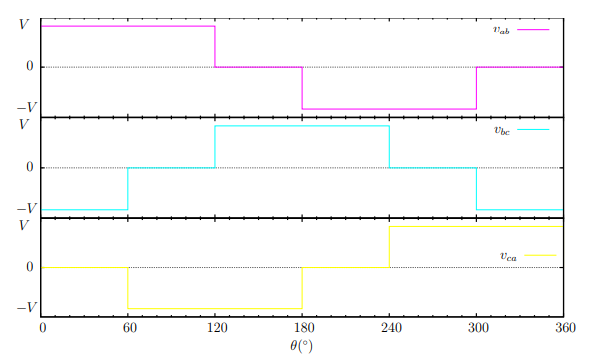
\includegraphics[width=0.32\textwidth]{imagens/grafico3_inversor_tri.png}
\caption{Acionamento dos transistores (à esquerda) da ponte inversora trifásica em operação seis pulsos 180º, assim como a tensão de fase (ao centro) e de linha (à direita) para a carga.}\label{g1it} 
\caption*{Fonte: Apostila de eletrônica de potência (2015)}
\end{figure}

Já o modo de comutação seis-pulsos 120º modifica o período de ativação de cada transistor para $\frac{2}{3}$ do período desejado, gerando intervalos de tensão não determinada, como pode ser visto na figura \ref{g4it}, estando os transistores em estado de alta impedância.
 
\begin{figure}[h]
\center
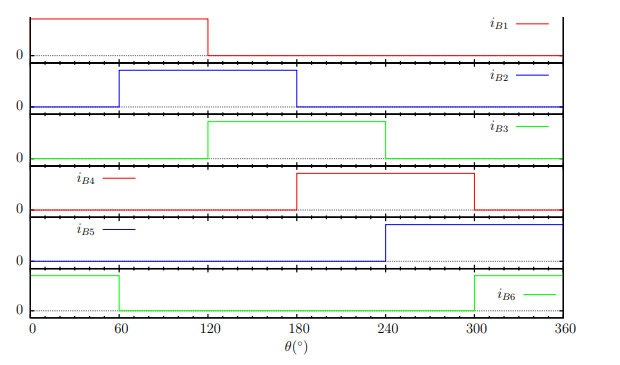
\includegraphics[width=0.32\textwidth]{imagens/grafico4_inversor_tri.png}
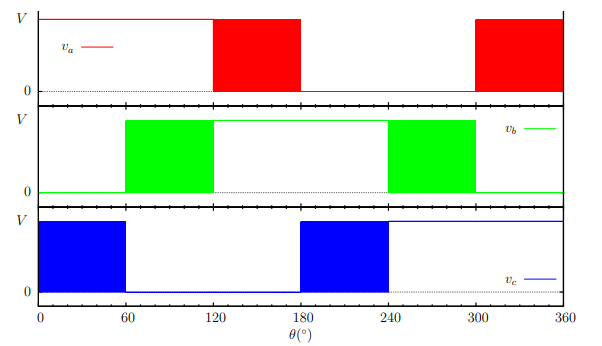
\includegraphics[width=0.32\textwidth]{imagens/grafico5_inversor_tri.png}
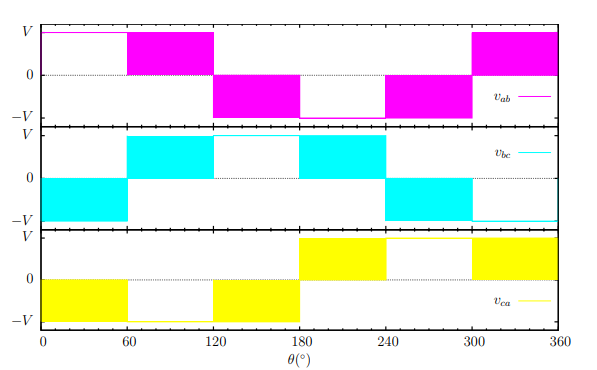
\includegraphics[width=0.32\textwidth]{imagens/grafico6_inversor_tri.png}
\caption{Acionamento dos transistores (à esquerda) da ponte inversora trifásica em operação seis pulsos 120º, assim como a tensão de fase (ao centro) e de linha (à direita) para a carga. Regiões sólidas representam um valor não determinado pelo inversor.}\label{g4it} 
\caption*{Fonte: Apostila de eletrônica de potência (2015)}
\end{figure}

Caso a carga seja puramente resistiva, a tensão aparente para essa será como ilustrado na figura \ref{g7it}. A tensão de linha (eficaz), então, torna-se \[
V_R = \frac{\sqrt{2} }{2}V
.\] 

 \begin{figure}[h]
\center
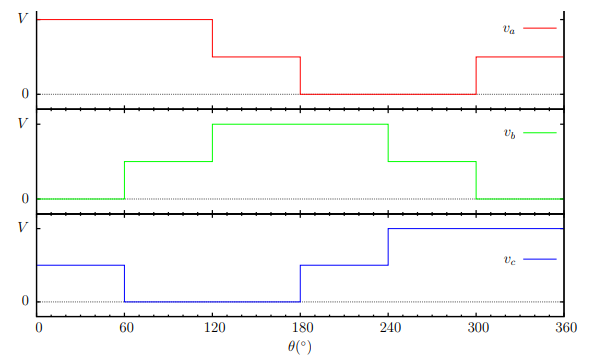
\includegraphics[width=0.45\textwidth]{imagens/grafico7_inversor_tri.png}
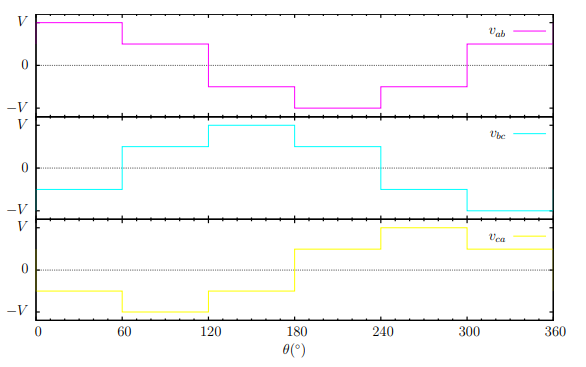
\includegraphics[width=0.45\textwidth]{imagens/grafico8_inversor_tri.png}
\caption{Tensão de fase (à esquerda) e linha (à direita) para uma carga resistiva em um inversor trifásico em modo de comutação seis-pontos 120º.}\label{g7it} 
\caption*{Fonte: Apostila de eletrônica de potência (2015)}
\end{figure}

